%
\begin{isabellebody}%
\setisabellecontext{FreeHOL}%
%
\isadelimtheory
%
\endisadelimtheory
%
\isatagtheory
%
\endisatagtheory
{\isafoldtheory}%
%
\isadelimtheory
%
\endisadelimtheory
%
\begin{isamarkuptext}%
\begin{abstract}
An embedding of free logic in classical higher-order logic is presented 
which has been formalized in Isabelle/HOL. Subsequently this 
work has been utilized as a foundation for the formalization of Peter Freyd's 
axiomatic category theory in Isabelle/HOL. Experiments with automated theorem provers integrated 
with Isabelle/HOL have been carried out, which revealed a previously unknown redundancy in 
Freyd's axiom system.
\end{abstract}%
\end{isamarkuptext}%
\isamarkuptrue%
%
\isamarkupsection{Free Logic%
}
\isamarkuptrue%
%
\begin{isamarkuptext}%
Motivated by problems and shortcomings in the handling of improper descriptions in the works of 
Russel, Frege and Hilbert-Bernays, the second author has proposed an alternative solution 
in his 1967 paper \emph{Existence and Description in Formal Logic} \cite{scott67:_exist}.

\begin{figure}
\newcommand\firstellipse{(2,-5) ellipse (6cm and 4cm)}
\newcommand\secondellipse{(0,-5) ellipse (4cm and 3cm)}
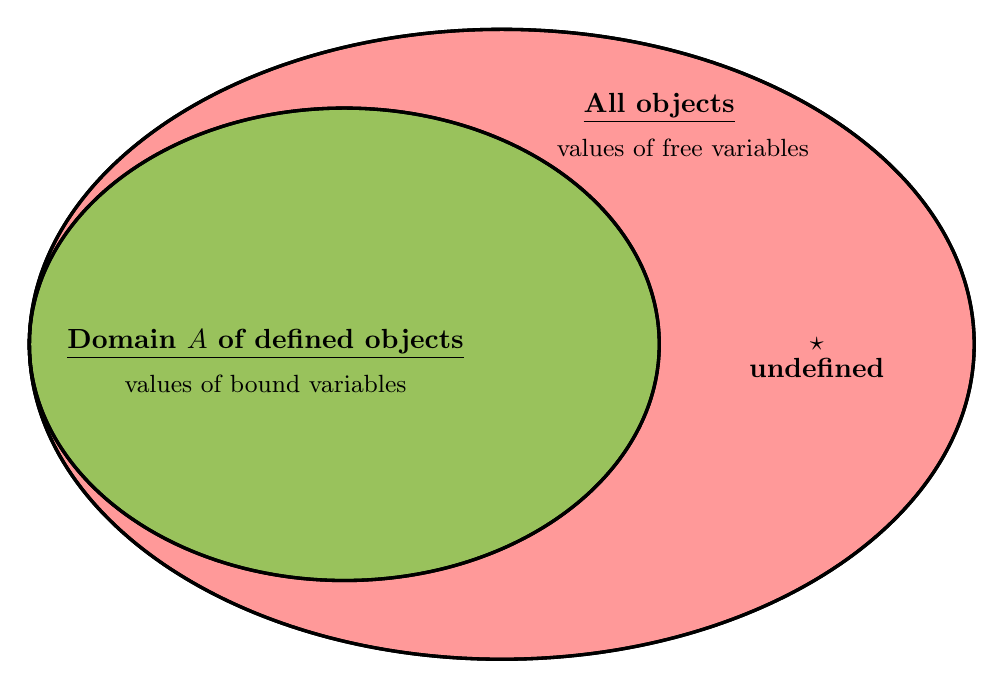
\begin{tikzpicture}
  \begin{scope}[fill opacity=0.4]
    \fill[red] \firstellipse;
    \fill[green] \secondellipse;
  \end{scope}
  \begin{scope}[very thick,font=\large]
    \draw \firstellipse node[font=\normalsize\bfseries] at (-1,-5) {\underline{Domain $\mathfrak{A}$ of defined objects}};
    \draw \firstellipse node[font=\small] at (-1,-5.5) {values of bound variables};
    \draw \secondellipse node[font=\normalsize\bfseries] at (4,-2) {\underline{All objects}};
    \draw \secondellipse node[font=\small] at (4.3,-2.5) {values of free variables};
  \end{scope}
  \node[font=\normalsize\bfseries] at (6,-5) {$\star$};
  \node[font=\normalsize\bfseries] at (6,-5.3) {undefined};
\end{tikzpicture}
\caption{Scott's Free Logic}
\end{figure}%
\end{isamarkuptext}%
\isamarkuptrue%
%
\isamarkupsection{Free Logic in HOL%
}
\isamarkuptrue%
%
\begin{isamarkuptext}%
In this section We present an embedding of the second authors \emph{Free Logic} in Isabelle/HOL.%
\end{isamarkuptext}%
\isamarkuptrue%
\isacommand{type{\isacharunderscore}synonym}\isamarkupfalse%
\ {\isasymsigma}\ {\isacharequal}\ {\isachardoublequoteopen}bool{\isachardoublequoteclose}\ \ \ %
\isamarkupcmt{the type for Booleans%
}
\ \ \ \isanewline
\isanewline
\isacommand{consts}\isamarkupfalse%
\ f{\isacharunderscore}A\ {\isacharcolon}{\isacharcolon}\ {\isachardoublequoteopen}{\isacharprime}a{\isasymRightarrow}{\isasymsigma}{\isachardoublequoteclose}\ {\isacharparenleft}{\isachardoublequoteopen}{\isasymA}{\isachardoublequoteclose}{\isacharparenright}\ \ \ \isanewline
\isacommand{consts}\isamarkupfalse%
\ f{\isacharunderscore}star\ {\isacharcolon}{\isacharcolon}\ {\isachardoublequoteopen}{\isacharprime}a{\isachardoublequoteclose}\ {\isacharparenleft}{\isachardoublequoteopen}\isactrlbold {\isasymstar}{\isachardoublequoteclose}{\isacharparenright}\ \ \ \isanewline
\isanewline
\isacommand{axiomatization}\isamarkupfalse%
\ \isakeyword{where}\ f{\isacharunderscore}star{\isacharunderscore}axiom{\isacharcolon}\ {\isachardoublequoteopen}{\isasymnot}{\isasymA}{\isacharparenleft}\isactrlbold {\isasymstar}{\isacharparenright}{\isachardoublequoteclose}\isanewline
\isanewline
\isacommand{axiomatization}\isamarkupfalse%
\ \isakeyword{where}\ non{\isacharunderscore}empty{\isacharcolon}\ {\isachardoublequoteopen}{\isasymexists}x{\isachardot}\ {\isasymA}{\isacharparenleft}x{\isacharparenright}\ {\isachardoublequoteclose}%
\begin{isamarkuptext}%
Negation and implication in free logic are mapped to negation in HOl.%
\end{isamarkuptext}%
\isamarkuptrue%
\isacommand{abbreviation}\isamarkupfalse%
\ f{\isacharunderscore}not\ {\isacharcolon}{\isacharcolon}\ {\isachardoublequoteopen}{\isasymsigma}{\isasymRightarrow}{\isasymsigma}{\isachardoublequoteclose}\ {\isacharparenleft}{\isachardoublequoteopen}\isactrlbold {\isasymnot}{\isacharunderscore}{\isachardoublequoteclose}\ {\isacharbrackleft}{\isadigit{5}}{\isadigit{8}}{\isacharbrackright}\ {\isadigit{5}}{\isadigit{9}}{\isacharparenright}\ \ \ \ \ \ \ \ \ \ \isanewline
\ \isakeyword{where}\ {\isachardoublequoteopen}\isactrlbold {\isasymnot}{\isasymphi}\ {\isasymequiv}\ {\isasymnot}{\isasymphi}{\isachardoublequoteclose}\ \ \ \ \ \isanewline
\isacommand{abbreviation}\isamarkupfalse%
\ f{\isacharunderscore}implies\ {\isacharcolon}{\isacharcolon}\ {\isachardoublequoteopen}{\isasymsigma}{\isasymRightarrow}{\isasymsigma}{\isasymRightarrow}{\isasymsigma}{\isachardoublequoteclose}\ {\isacharparenleft}\isakeyword{infixr}\ {\isachardoublequoteopen}\isactrlbold {\isasymrightarrow}{\isachardoublequoteclose}\ {\isadigit{4}}{\isadigit{9}}{\isacharparenright}\ \ \ \isanewline
\ \isakeyword{where}\ {\isachardoublequoteopen}{\isasymphi}\isactrlbold {\isasymrightarrow}{\isasympsi}\ {\isasymequiv}\ {\isasymphi}{\isasymlongrightarrow}{\isasympsi}{\isachardoublequoteclose}%
\begin{isamarkuptext}%
Universal quantification in free logic is restricted to the domain of existing objects%
\end{isamarkuptext}%
\isamarkuptrue%
\isacommand{abbreviation}\isamarkupfalse%
\ f{\isacharunderscore}all\ {\isacharcolon}{\isacharcolon}\ {\isachardoublequoteopen}{\isacharparenleft}{\isacharprime}a{\isasymRightarrow}{\isasymsigma}{\isacharparenright}{\isasymRightarrow}{\isasymsigma}{\isachardoublequoteclose}\ {\isacharparenleft}{\isachardoublequoteopen}\isactrlbold {\isasymforall}{\isachardoublequoteclose}{\isacharparenright}\ \ \ \ \ \ \ \ \ \ \ \ \ \ \ \ \ \isanewline
\ \isakeyword{where}\ {\isachardoublequoteopen}\isactrlbold {\isasymforall}{\isasymPhi}\ {\isasymequiv}\ {\isasymforall}x{\isachardot}\ {\isasymA}{\isacharparenleft}x{\isacharparenright}{\isasymlongrightarrow}{\isasymPhi}{\isacharparenleft}x{\isacharparenright}{\isachardoublequoteclose}\ \ \ \isanewline
\isacommand{abbreviation}\isamarkupfalse%
\ f{\isacharunderscore}all{\isacharunderscore}bind\ {\isacharcolon}{\isacharcolon}\ {\isachardoublequoteopen}{\isacharparenleft}{\isacharprime}a{\isasymRightarrow}{\isasymsigma}{\isacharparenright}{\isasymRightarrow}{\isasymsigma}{\isachardoublequoteclose}\ {\isacharparenleft}\isakeyword{binder}\ {\isachardoublequoteopen}\isactrlbold {\isasymforall}{\isachardoublequoteclose}\ {\isacharbrackleft}{\isadigit{8}}{\isacharbrackright}\ {\isadigit{9}}{\isacharparenright}\ \isanewline
\ \isakeyword{where}\ {\isachardoublequoteopen}\isactrlbold {\isasymforall}x{\isachardot}\ {\isasymphi}{\isacharparenleft}x{\isacharparenright}\ {\isasymequiv}\ \isactrlbold {\isasymforall}{\isasymphi}{\isachardoublequoteclose}\isanewline
\isacommand{abbreviation}\isamarkupfalse%
\ f{\isacharunderscore}that\ {\isacharcolon}{\isacharcolon}\ {\isachardoublequoteopen}{\isacharparenleft}{\isacharprime}a{\isasymRightarrow}{\isasymsigma}{\isacharparenright}{\isasymRightarrow}{\isacharprime}a{\isachardoublequoteclose}\ {\isacharparenleft}{\isachardoublequoteopen}\isactrlbold I{\isachardoublequoteclose}{\isacharparenright}\ \isanewline
\ \isakeyword{where}\ {\isachardoublequoteopen}\isactrlbold I\ {\isasymPhi}\ {\isasymequiv}\ if\ {\isasymexists}x{\isachardot}\ {\isasymA}{\isacharparenleft}x{\isacharparenright}\ {\isasymand}\ {\isasymPhi}{\isacharparenleft}x{\isacharparenright}\ {\isasymand}\ {\isacharparenleft}{\isasymforall}y{\isachardot}\ {\isacharparenleft}{\isasymA}{\isacharparenleft}y{\isacharparenright}\ {\isasymand}\ {\isasymPhi}{\isacharparenleft}y{\isacharparenright}{\isacharparenright}\ {\isasymlongrightarrow}\ {\isacharparenleft}y\ {\isacharequal}\ x{\isacharparenright}{\isacharparenright}\ \isanewline
\ \ \ \ \ \ \ \ \ \ \ \ \ \ \ then\ THE\ x{\isachardot}\ {\isasymA}{\isacharparenleft}x{\isacharparenright}\ {\isasymand}\ {\isasymPhi}{\isacharparenleft}x{\isacharparenright}\ \isanewline
\ \ \ \ \ \ \ \ \ \ \ \ \ \ \ else\ \isactrlbold {\isasymstar}{\isachardoublequoteclose}\isanewline
\isacommand{abbreviation}\isamarkupfalse%
\ f{\isacharunderscore}that{\isacharunderscore}b\ {\isacharcolon}{\isacharcolon}\ {\isachardoublequoteopen}{\isacharparenleft}{\isacharprime}a{\isasymRightarrow}{\isasymsigma}{\isacharparenright}{\isasymRightarrow}{\isacharprime}a{\isachardoublequoteclose}\ \ {\isacharparenleft}\isakeyword{binder}\ {\isachardoublequoteopen}\isactrlbold I{\isachardoublequoteclose}\ {\isacharbrackleft}{\isadigit{8}}{\isacharbrackright}\ {\isadigit{9}}{\isacharparenright}\ \isanewline
\ \isakeyword{where}\ {\isachardoublequoteopen}\isactrlbold Ix{\isachardot}\ {\isasymphi}{\isacharparenleft}x{\isacharparenright}\ {\isasymequiv}\ \isactrlbold I{\isacharparenleft}{\isasymphi}{\isacharparenright}{\isachardoublequoteclose}\isanewline
\isanewline
\isanewline
\isanewline
\isacommand{abbreviation}\isamarkupfalse%
\ f{\isacharunderscore}or\ {\isacharcolon}{\isacharcolon}\ {\isachardoublequoteopen}{\isasymsigma}{\isasymRightarrow}{\isasymsigma}{\isasymRightarrow}{\isasymsigma}{\isachardoublequoteclose}\ {\isacharparenleft}\isakeyword{infixr}\ {\isachardoublequoteopen}\isactrlbold {\isasymor}{\isachardoublequoteclose}\ {\isadigit{5}}{\isadigit{1}}{\isacharparenright}\ \ \ \ \ \ \ \ \ \isanewline
\ \isakeyword{where}\ {\isachardoublequoteopen}{\isasymphi}\isactrlbold {\isasymor}{\isasympsi}\ {\isasymequiv}\ {\isacharparenleft}\isactrlbold {\isasymnot}{\isasymphi}{\isacharparenright}\isactrlbold {\isasymrightarrow}{\isasympsi}{\isachardoublequoteclose}\ \isanewline
\isacommand{abbreviation}\isamarkupfalse%
\ f{\isacharunderscore}and\ {\isacharcolon}{\isacharcolon}\ {\isachardoublequoteopen}{\isasymsigma}{\isasymRightarrow}{\isasymsigma}{\isasymRightarrow}{\isasymsigma}{\isachardoublequoteclose}\ {\isacharparenleft}\isakeyword{infixr}\ {\isachardoublequoteopen}\isactrlbold {\isasymand}{\isachardoublequoteclose}\ {\isadigit{5}}{\isadigit{2}}{\isacharparenright}\ \ \ \ \ \ \ \ \isanewline
\ \isakeyword{where}\ {\isachardoublequoteopen}{\isasymphi}\isactrlbold {\isasymand}{\isasympsi}\ {\isasymequiv}\ \isactrlbold {\isasymnot}{\isacharparenleft}\isactrlbold {\isasymnot}{\isasymphi}\isactrlbold {\isasymor}\isactrlbold {\isasymnot}{\isasympsi}{\isacharparenright}{\isachardoublequoteclose}\ \ \ \ \isanewline
\isacommand{abbreviation}\isamarkupfalse%
\ f{\isacharunderscore}equiv\ {\isacharcolon}{\isacharcolon}\ {\isachardoublequoteopen}{\isasymsigma}{\isasymRightarrow}{\isasymsigma}{\isasymRightarrow}{\isasymsigma}{\isachardoublequoteclose}\ {\isacharparenleft}\isakeyword{infixr}\ {\isachardoublequoteopen}\isactrlbold {\isasymleftrightarrow}{\isachardoublequoteclose}\ {\isadigit{5}}{\isadigit{0}}{\isacharparenright}\ \ \ \ \ \isanewline
\ \isakeyword{where}\ {\isachardoublequoteopen}{\isasymphi}\isactrlbold {\isasymleftrightarrow}{\isasympsi}\ {\isasymequiv}\ {\isacharparenleft}{\isasymphi}\isactrlbold {\isasymrightarrow}{\isasympsi}{\isacharparenright}\isactrlbold {\isasymand}{\isacharparenleft}{\isasympsi}\isactrlbold {\isasymrightarrow}{\isasymphi}{\isacharparenright}{\isachardoublequoteclose}\ \ \isanewline
\isacommand{abbreviation}\isamarkupfalse%
\ f{\isacharunderscore}equals\ {\isacharcolon}{\isacharcolon}\ {\isachardoublequoteopen}{\isacharprime}a{\isasymRightarrow}{\isacharprime}a{\isasymRightarrow}{\isasymsigma}{\isachardoublequoteclose}\ {\isacharparenleft}\isakeyword{infixr}\ {\isachardoublequoteopen}\isactrlbold {\isacharequal}{\isachardoublequoteclose}{\isadigit{5}}{\isadigit{6}}{\isacharparenright}\ \ \ \ \ \ \ \isanewline
\ \isakeyword{where}\ {\isachardoublequoteopen}x\isactrlbold {\isacharequal}y\ {\isasymequiv}\ x{\isacharequal}y{\isachardoublequoteclose}\isanewline
\isacommand{abbreviation}\isamarkupfalse%
\ f{\isacharunderscore}exi\ {\isacharcolon}{\isacharcolon}\ {\isachardoublequoteopen}{\isacharparenleft}{\isacharprime}a{\isasymRightarrow}{\isasymsigma}{\isacharparenright}{\isasymRightarrow}{\isasymsigma}{\isachardoublequoteclose}\ {\isacharparenleft}{\isachardoublequoteopen}\isactrlbold {\isasymexists}{\isachardoublequoteclose}{\isacharparenright}\ \ \ \ \ \ \ \ \ \ \ \ \ \ \ \ \ \isanewline
\ \isakeyword{where}\ {\isachardoublequoteopen}\isactrlbold {\isasymexists}{\isasymPhi}\ {\isasymequiv}\ \isactrlbold {\isasymnot}\isactrlbold {\isasymforall}{\isacharparenleft}{\isasymlambda}y{\isachardot}\isactrlbold {\isasymnot}{\isacharparenleft}{\isasymPhi}\ y{\isacharparenright}{\isacharparenright}{\isachardoublequoteclose}\isanewline
\isacommand{abbreviation}\isamarkupfalse%
\ f{\isacharunderscore}exi{\isacharunderscore}b\ {\isacharcolon}{\isacharcolon}\ {\isachardoublequoteopen}{\isacharparenleft}{\isacharprime}a{\isasymRightarrow}{\isasymsigma}{\isacharparenright}{\isasymRightarrow}{\isasymsigma}{\isachardoublequoteclose}\ \ {\isacharparenleft}\isakeyword{binder}\ {\isachardoublequoteopen}\isactrlbold {\isasymexists}{\isachardoublequoteclose}\ {\isacharbrackleft}{\isadigit{8}}{\isacharbrackright}{\isadigit{9}}{\isacharparenright}\ \ \isanewline
\ \isakeyword{where}\ {\isachardoublequoteopen}\isactrlbold {\isasymexists}x{\isachardot}\ {\isasymphi}{\isacharparenleft}x{\isacharparenright}\ {\isasymequiv}\ \isactrlbold {\isasymexists}{\isasymphi}{\isachardoublequoteclose}%
\isamarkupsection{Some Introductory Tests%
}
\isamarkuptrue%
%
\isamarkupcmt{See Scott, Existence and Description in Formal Logic, 1967, pages 183-184%
}
\isanewline
\isanewline
\isacommand{typedecl}\isamarkupfalse%
\ {\isasymiota}\ \ \ \ \ \ \ \ \ \ \ \ \ \ \ \ %
\isamarkupcmt{the type for indiviuals%
}
\ \ \isanewline
\isacommand{consts}\isamarkupfalse%
\ f{\isacharunderscore}r\ \ {\isacharcolon}{\isacharcolon}\ {\isachardoublequoteopen}{\isasymiota}{\isasymRightarrow}{\isasymiota}{\isasymRightarrow}{\isasymsigma}{\isachardoublequoteclose}\ {\isacharparenleft}\isakeyword{infixr}\ {\isachardoublequoteopen}\isactrlbold r{\isachardoublequoteclose}\ {\isadigit{7}}{\isadigit{0}}{\isacharparenright}\ \ \ \ \ \isanewline
\isanewline
\isacommand{lemma}\isamarkupfalse%
\ {\isachardoublequoteopen}x\ \isactrlbold r\ x\ \isactrlbold {\isasymrightarrow}\ x\ \isactrlbold r\ x{\isachardoublequoteclose}%
\isadelimproof
\ %
\endisadelimproof
%
\isatagproof
\isacommand{by}\isamarkupfalse%
\ simp%
\endisatagproof
{\isafoldproof}%
%
\isadelimproof
%
\endisadelimproof
\ \ \isanewline
\ \isanewline
\isacommand{lemma}\isamarkupfalse%
\ {\isachardoublequoteopen}\isactrlbold {\isasymexists}y{\isachardot}\ y\ \isactrlbold r\ y\ \isactrlbold {\isasymrightarrow}\ y\ \isactrlbold r\ y{\isachardoublequoteclose}\ \isacommand{nitpick}\isamarkupfalse%
%
\isadelimproof
\ %
\endisadelimproof
%
\isatagproof
\isacommand{oops}\isamarkupfalse%
%
\endisatagproof
{\isafoldproof}%
%
\isadelimproof
%
\endisadelimproof
\ \ \ \ \isanewline
\ \isanewline
\isacommand{lemma}\isamarkupfalse%
\ {\isachardoublequoteopen}{\isacharparenleft}x\ \isactrlbold r\ x\ \isactrlbold {\isasymrightarrow}\ x\ \isactrlbold r\ x{\isacharparenright}\ \isactrlbold {\isasymrightarrow}\ {\isacharparenleft}\isactrlbold {\isasymexists}y{\isachardot}\ y\ \isactrlbold r\ y\ \isactrlbold {\isasymrightarrow}\ y\ \isactrlbold r\ y{\isacharparenright}{\isachardoublequoteclose}\ \isacommand{nitpick}\isamarkupfalse%
%
\isadelimproof
\ %
\endisadelimproof
%
\isatagproof
\isacommand{oops}\isamarkupfalse%
%
\endisatagproof
{\isafoldproof}%
%
\isadelimproof
%
\endisadelimproof
\isanewline
\ \isanewline
\isacommand{lemma}\isamarkupfalse%
\ {\isachardoublequoteopen}{\isacharparenleft}{\isacharparenleft}x\ \isactrlbold r\ x\ \isactrlbold {\isasymrightarrow}\ x\ \isactrlbold r\ x{\isacharparenright}\ \isactrlbold {\isasymand}\ {\isacharparenleft}\isactrlbold {\isasymexists}y{\isacharcolon}{\isacharcolon}{\isasymiota}{\isachardot}\ y\ \isactrlbold {\isacharequal}\ y{\isacharparenright}{\isacharparenright}\ \isactrlbold {\isasymrightarrow}\ {\isacharparenleft}\isactrlbold {\isasymexists}y{\isachardot}\ y\ \isactrlbold r\ y\ \isactrlbold {\isasymrightarrow}\ y\ \isactrlbold r\ y{\isacharparenright}{\isachardoublequoteclose}%
\isadelimproof
\ %
\endisadelimproof
%
\isatagproof
\isacommand{by}\isamarkupfalse%
\ simp\isanewline
\ \isanewline
\isanewline
\isanewline
%
\isamarkupcmt{See Scott 1967, page 185%
}
%
\endisatagproof
{\isafoldproof}%
%
\isadelimproof
%
\endisadelimproof
\isanewline
\isacommand{lemma}\isamarkupfalse%
\ S{\isadigit{1}}{\isacharunderscore}inst\ {\isacharcolon}\ {\isachardoublequoteopen}{\isacharparenleft}\isactrlbold {\isasymforall}x{\isachardot}\ {\isasymPhi}{\isacharparenleft}x{\isacharparenright}\ \isactrlbold {\isasymrightarrow}\ {\isasymPsi}{\isacharparenleft}x{\isacharparenright}{\isacharparenright}\ \isactrlbold {\isasymrightarrow}\ {\isacharparenleft}{\isacharparenleft}\isactrlbold {\isasymforall}x{\isachardot}\ {\isasymPhi}{\isacharparenleft}x{\isacharparenright}{\isacharparenright}\ \isactrlbold {\isasymrightarrow}\ {\isacharparenleft}\isactrlbold {\isasymforall}x{\isachardot}\ {\isasymPsi}{\isacharparenleft}x{\isacharparenright}{\isacharparenright}{\isacharparenright}{\isachardoublequoteclose}%
\isadelimproof
\ %
\endisadelimproof
%
\isatagproof
\isacommand{by}\isamarkupfalse%
\ auto%
\endisatagproof
{\isafoldproof}%
%
\isadelimproof
%
\endisadelimproof
\isanewline
\isacommand{lemma}\isamarkupfalse%
\ S{\isadigit{2}}\ {\isacharcolon}\ \ \ \ \ \ {\isachardoublequoteopen}\isactrlbold {\isasymforall}y{\isachardot}\ \isactrlbold {\isasymexists}x{\isachardot}\ x\ \isactrlbold {\isacharequal}\ y{\isachardoublequoteclose}%
\isadelimproof
\ %
\endisadelimproof
%
\isatagproof
\isacommand{by}\isamarkupfalse%
\ auto%
\endisatagproof
{\isafoldproof}%
%
\isadelimproof
%
\endisadelimproof
\isanewline
\isacommand{lemma}\isamarkupfalse%
\ S{\isadigit{3}}\ {\isacharcolon}\ \ \ \ \ \ {\isachardoublequoteopen}{\isasymalpha}\ \isactrlbold {\isacharequal}\ {\isasymalpha}{\isachardoublequoteclose}%
\isadelimproof
\ %
\endisadelimproof
%
\isatagproof
\isacommand{by}\isamarkupfalse%
\ auto%
\endisatagproof
{\isafoldproof}%
%
\isadelimproof
%
\endisadelimproof
\isanewline
\isacommand{lemma}\isamarkupfalse%
\ S{\isadigit{4}}{\isacharunderscore}inst\ {\isacharcolon}\ {\isachardoublequoteopen}{\isacharparenleft}{\isasymPhi}{\isacharparenleft}{\isasymalpha}{\isacharparenright}\ \isactrlbold {\isasymand}\ {\isacharparenleft}{\isasymalpha}\ \isactrlbold {\isacharequal}\ {\isasymbeta}{\isacharparenright}{\isacharparenright}\ \isactrlbold {\isasymrightarrow}\ {\isasymPhi}{\isacharparenleft}{\isasymbeta}{\isacharparenright}{\isachardoublequoteclose}%
\isadelimproof
\ %
\endisadelimproof
%
\isatagproof
\isacommand{by}\isamarkupfalse%
\ auto%
\endisatagproof
{\isafoldproof}%
%
\isadelimproof
%
\endisadelimproof
\isanewline
\isacommand{lemma}\isamarkupfalse%
\ UI{\isacharunderscore}inst\ {\isacharcolon}\ {\isachardoublequoteopen}{\isacharparenleft}{\isacharparenleft}\isactrlbold {\isasymforall}x{\isachardot}\ {\isasymPhi}{\isacharparenleft}x{\isacharparenright}{\isacharparenright}\ \isactrlbold {\isasymand}\ {\isacharparenleft}\isactrlbold {\isasymexists}x{\isachardot}\ x\ \isactrlbold {\isacharequal}\ {\isasymalpha}{\isacharparenright}{\isacharparenright}\ \isactrlbold {\isasymrightarrow}\ {\isasymPhi}{\isacharparenleft}{\isasymalpha}{\isacharparenright}{\isachardoublequoteclose}%
\isadelimproof
\ %
\endisadelimproof
%
\isatagproof
\isacommand{by}\isamarkupfalse%
\ auto%
\endisatagproof
{\isafoldproof}%
%
\isadelimproof
%
\endisadelimproof
\isanewline
\isacommand{lemma}\isamarkupfalse%
\ UI{\isacharunderscore}test\ {\isacharcolon}\ {\isachardoublequoteopen}{\isacharparenleft}\isactrlbold {\isasymforall}x{\isachardot}\ {\isasymPhi}{\isacharparenleft}x{\isacharparenright}{\isacharparenright}\ \isactrlbold {\isasymrightarrow}\ {\isasymPhi}{\isacharparenleft}{\isasymalpha}{\isacharparenright}{\isachardoublequoteclose}\ \isacommand{nitpick}\isamarkupfalse%
\ {\isacharbrackleft}user{\isacharunderscore}axioms{\isacharbrackright}%
\isadelimproof
\ %
\endisadelimproof
%
\isatagproof
\isacommand{oops}\isamarkupfalse%
\ %
\isamarkupcmt{Countermodel%
}
%
\endisatagproof
{\isafoldproof}%
%
\isadelimproof
%
\endisadelimproof
\isanewline
\isacommand{lemma}\isamarkupfalse%
\ UI{\isacharunderscore}cor{\isadigit{1}}\ {\isacharcolon}\ {\isachardoublequoteopen}\isactrlbold {\isasymforall}y{\isachardot}{\isacharparenleft}{\isacharparenleft}\isactrlbold {\isasymforall}x{\isachardot}\ {\isasymPhi}{\isacharparenleft}x{\isacharparenright}{\isacharparenright}\ \isactrlbold {\isasymrightarrow}\ {\isasymPhi}{\isacharparenleft}y{\isacharparenright}{\isacharparenright}{\isachardoublequoteclose}%
\isadelimproof
\ %
\endisadelimproof
%
\isatagproof
\isacommand{by}\isamarkupfalse%
\ auto%
\endisatagproof
{\isafoldproof}%
%
\isadelimproof
%
\endisadelimproof
\isanewline
\isacommand{lemma}\isamarkupfalse%
\ UI{\isacharunderscore}cor{\isadigit{2}}\ {\isacharcolon}\ {\isachardoublequoteopen}\isactrlbold {\isasymforall}y{\isachardot}{\isacharparenleft}{\isacharparenleft}\isactrlbold {\isasymforall}x{\isachardot}\ \isactrlbold {\isasymnot}{\isacharparenleft}x\ \isactrlbold {\isacharequal}\ y{\isacharparenright}{\isacharparenright}\ \isactrlbold {\isasymrightarrow}\ \isactrlbold {\isasymnot}{\isacharparenleft}y\ \isactrlbold {\isacharequal}\ y{\isacharparenright}{\isacharparenright}{\isachardoublequoteclose}%
\isadelimproof
\ %
\endisadelimproof
%
\isatagproof
\isacommand{by}\isamarkupfalse%
\ auto%
\endisatagproof
{\isafoldproof}%
%
\isadelimproof
%
\endisadelimproof
\isanewline
\isacommand{lemma}\isamarkupfalse%
\ UI{\isacharunderscore}cor{\isadigit{3}}\ {\isacharcolon}\ {\isachardoublequoteopen}\isactrlbold {\isasymforall}y{\isachardot}{\isacharparenleft}{\isacharparenleft}y\ \isactrlbold {\isacharequal}\ y{\isacharparenright}\ \isactrlbold {\isasymrightarrow}\ {\isacharparenleft}\isactrlbold {\isasymexists}x{\isachardot}\ x\ \isactrlbold {\isacharequal}\ y{\isacharparenright}{\isacharparenright}{\isachardoublequoteclose}%
\isadelimproof
\ %
\endisadelimproof
%
\isatagproof
\isacommand{by}\isamarkupfalse%
\ auto%
\endisatagproof
{\isafoldproof}%
%
\isadelimproof
%
\endisadelimproof
\isanewline
\isacommand{lemma}\isamarkupfalse%
\ UI{\isacharunderscore}cor{\isadigit{4}}\ {\isacharcolon}\ {\isachardoublequoteopen}{\isacharparenleft}\isactrlbold {\isasymforall}y{\isachardot}\ y\ \isactrlbold {\isacharequal}\ y{\isacharparenright}\ \isactrlbold {\isasymrightarrow}\ {\isacharparenleft}\isactrlbold {\isasymforall}y{\isachardot}\isactrlbold {\isasymexists}x{\isachardot}\ x\ \isactrlbold {\isacharequal}\ y{\isacharparenright}{\isachardoublequoteclose}%
\isadelimproof
\ %
\endisadelimproof
%
\isatagproof
\isacommand{by}\isamarkupfalse%
\ simp%
\endisatagproof
{\isafoldproof}%
%
\isadelimproof
%
\endisadelimproof
\isanewline
\isanewline
\isacommand{lemma}\isamarkupfalse%
\ {\isachardoublequoteopen}{\isacharparenleft}\isactrlbold {\isasymexists}x{\isachardot}\ x\ \isactrlbold {\isacharequal}\ {\isasymalpha}{\isacharparenright}\ {\isasymlongrightarrow}\ {\isasymA}{\isacharparenleft}{\isasymalpha}{\isacharparenright}{\isachardoublequoteclose}%
\isadelimproof
\ %
\endisadelimproof
%
\isatagproof
\isacommand{by}\isamarkupfalse%
\ simp%
\endisatagproof
{\isafoldproof}%
%
\isadelimproof
%
\endisadelimproof
\isanewline
\ \isanewline
\isanewline
\isanewline
\isacommand{lemma}\isamarkupfalse%
\ I{\isadigit{1}}{\isacharunderscore}inst\ {\isacharcolon}\ {\isachardoublequoteopen}\isactrlbold {\isasymforall}y{\isachardot}\ {\isacharparenleft}{\isacharparenleft}y\ \isactrlbold {\isacharequal}\ {\isacharparenleft}\isactrlbold Ix{\isachardot}\ {\isasymPhi}{\isacharparenleft}x{\isacharparenright}{\isacharparenright}{\isacharparenright}\ \isactrlbold {\isasymleftrightarrow}\ {\isacharparenleft}\isactrlbold {\isasymforall}x{\isachardot}\ {\isacharparenleft}{\isacharparenleft}x\ \isactrlbold {\isacharequal}\ y{\isacharparenright}\ \isactrlbold {\isasymleftrightarrow}\ {\isasymPhi}{\isacharparenleft}x{\isacharparenright}{\isacharparenright}{\isacharparenright}{\isacharparenright}{\isachardoublequoteclose}%
\isadelimproof
\ %
\endisadelimproof
%
\isatagproof
\isacommand{by}\isamarkupfalse%
\ {\isacharparenleft}smt\ f{\isacharunderscore}star{\isacharunderscore}axiom\ the{\isacharunderscore}equality{\isacharparenright}%
\endisatagproof
{\isafoldproof}%
%
\isadelimproof
%
\endisadelimproof
\isanewline
\isanewline
\isanewline
\isacommand{abbreviation}\isamarkupfalse%
\ star\ {\isacharparenleft}{\isachardoublequoteopen}{\isasymOtimes}{\isachardoublequoteclose}{\isacharparenright}\ \isakeyword{where}\ {\isachardoublequoteopen}{\isasymOtimes}\ {\isasymequiv}\ \isactrlbold Iy{\isachardot}\ \isactrlbold {\isasymnot}\ {\isacharparenleft}y\ \isactrlbold {\isacharequal}\ y{\isacharparenright}{\isachardoublequoteclose}\isanewline
\isanewline
\isacommand{lemma}\isamarkupfalse%
\ test\ {\isacharcolon}\ {\isachardoublequoteopen}{\isasymOtimes}\ {\isacharequal}\ \isactrlbold {\isasymstar}{\isachardoublequoteclose}%
\isadelimproof
\ %
\endisadelimproof
%
\isatagproof
\isacommand{by}\isamarkupfalse%
\ simp%
\endisatagproof
{\isafoldproof}%
%
\isadelimproof
%
\endisadelimproof
\isanewline
\isanewline
\isanewline
\isacommand{lemma}\isamarkupfalse%
\ I{\isadigit{2}}{\isacharunderscore}inst\ {\isacharcolon}\ {\isachardoublequoteopen}\isactrlbold {\isasymnot}{\isacharparenleft}\isactrlbold {\isasymexists}y{\isachardot}\ y\ \isactrlbold {\isacharequal}\ {\isacharparenleft}\isactrlbold Ix{\isachardot}\ {\isasymPhi}{\isacharparenleft}x{\isacharparenright}{\isacharparenright}{\isacharparenright}\ \isactrlbold {\isasymrightarrow}\ \ {\isacharparenleft}{\isasymOtimes}\ \isactrlbold {\isacharequal}\ {\isacharparenleft}\isactrlbold Ix{\isachardot}\ {\isasymPhi}{\isacharparenleft}x{\isacharparenright}{\isacharparenright}{\isacharparenright}{\isachardoublequoteclose}%
\isadelimproof
\ %
\endisadelimproof
%
\isatagproof
\isacommand{by}\isamarkupfalse%
\ {\isacharparenleft}metis\ {\isacharparenleft}no{\isacharunderscore}types{\isacharcomma}\ lifting{\isacharparenright}\ the{\isacharunderscore}equality{\isacharparenright}%
\endisatagproof
{\isafoldproof}%
%
\isadelimproof
%
\endisadelimproof
\isanewline
\isanewline
\ \isanewline
\isacommand{lemma}\isamarkupfalse%
\ Ext{\isacharunderscore}inst\ {\isacharcolon}\ {\isachardoublequoteopen}{\isacharparenleft}\isactrlbold {\isasymforall}x{\isachardot}\ {\isasymPhi}{\isacharparenleft}x{\isacharparenright}\ \isactrlbold {\isasymleftrightarrow}\ {\isasymPsi}{\isacharparenleft}x{\isacharparenright}{\isacharparenright}\ \isactrlbold {\isasymrightarrow}\ {\isacharparenleft}{\isacharparenleft}\isactrlbold Ix{\isachardot}\ {\isasymPhi}{\isacharparenleft}x{\isacharparenright}{\isacharparenright}\ \isactrlbold {\isacharequal}\ {\isacharparenleft}\isactrlbold Ix{\isachardot}\ {\isasymPsi}{\isacharparenleft}x{\isacharparenright}{\isacharparenright}{\isacharparenright}{\isachardoublequoteclose}%
\isadelimproof
\ %
\endisadelimproof
%
\isatagproof
\isacommand{by}\isamarkupfalse%
\ {\isacharparenleft}smt\ the{\isadigit{1}}{\isacharunderscore}equality{\isacharparenright}%
\endisatagproof
{\isafoldproof}%
%
\isadelimproof
%
\endisadelimproof
\isanewline
\isanewline
\isanewline
\ \isanewline
\isacommand{lemma}\isamarkupfalse%
\ I{\isadigit{3}}\ {\isacharcolon}\ {\isachardoublequoteopen}{\isacharparenleft}{\isasymOtimes}\ \isactrlbold {\isacharequal}\ {\isasymalpha}\ \isactrlbold {\isasymor}\ {\isasymOtimes}\ \isactrlbold {\isacharequal}\ {\isasymbeta}{\isacharparenright}\ \isactrlbold {\isasymrightarrow}\ \isactrlbold {\isasymnot}{\isacharparenleft}{\isasymalpha}\ \isactrlbold r\ {\isasymbeta}{\isacharparenright}{\isachardoublequoteclose}\ \isacommand{nitpick}\isamarkupfalse%
\ {\isacharbrackleft}user{\isacharunderscore}axioms{\isacharbrackright}%
\isadelimproof
\ %
\endisadelimproof
%
\isatagproof
\isacommand{oops}\isamarkupfalse%
%
\endisatagproof
{\isafoldproof}%
%
\isadelimproof
%
\endisadelimproof
\isanewline
\isanewline
\isanewline
\ \isanewline
\isacommand{lemma}\isamarkupfalse%
\ Russel{\isacharunderscore}inst\ {\isacharcolon}\ \isanewline
\ {\isachardoublequoteopen}{\isacharparenleft}{\isacharparenleft}{\isasymOtimes}\ \isactrlbold {\isacharequal}\ {\isasymalpha}\ \isactrlbold {\isasymor}\ {\isasymOtimes}\ \isactrlbold {\isacharequal}\ {\isasymbeta}{\isacharparenright}\ \isactrlbold {\isasymrightarrow}\ \isactrlbold {\isasymnot}{\isacharparenleft}{\isasymalpha}\ \isactrlbold r\ {\isasymbeta}{\isacharparenright}{\isacharparenright}\ \isanewline
\ \ \isactrlbold {\isasymrightarrow}\ \isanewline
\ \ {\isacharparenleft}{\isacharparenleft}{\isasymalpha}\ \isactrlbold r\ {\isacharparenleft}\isactrlbold Ix{\isachardot}\ {\isasymPhi}{\isacharparenleft}x{\isacharparenright}{\isacharparenright}{\isacharparenright}\ \isactrlbold {\isasymleftrightarrow}\ {\isacharparenleft}\isactrlbold {\isasymexists}y{\isachardot}{\isacharparenleft}{\isacharparenleft}\isactrlbold {\isasymforall}x{\isachardot}\ {\isacharparenleft}{\isacharparenleft}x\ \isactrlbold {\isacharequal}\ y{\isacharparenright}\ \isactrlbold {\isasymleftrightarrow}\ {\isasymPhi}{\isacharparenleft}x{\isacharparenright}{\isacharparenright}{\isacharparenright}\ \isactrlbold {\isasymand}\ {\isacharparenleft}{\isasymalpha}\ \isactrlbold r\ y{\isacharparenright}{\isacharparenright}{\isacharparenright}{\isacharparenright}{\isachardoublequoteclose}\isanewline
\isacommand{nitpick}\isamarkupfalse%
\ {\isacharbrackleft}user{\isacharunderscore}axioms{\isacharbrackright}%
\isadelimproof
\ %
\endisadelimproof
%
\isatagproof
\isacommand{oops}\isamarkupfalse%
%
\endisatagproof
{\isafoldproof}%
%
\isadelimproof
%
\endisadelimproof
\isanewline
\isanewline
\isanewline
\isanewline
\isanewline
\isacommand{lemma}\isamarkupfalse%
\ {\isachardoublequoteopen}\isactrlbold {\isasymnot}{\isacharparenleft}\isactrlbold {\isasymexists}x{\isachardot}\ {\isacharparenleft}x\ \isactrlbold {\isacharequal}\ {\isacharparenleft}\isactrlbold Iy{\isachardot}\ \isactrlbold {\isasymnot}\ {\isacharparenleft}y\ \isactrlbold {\isacharequal}\ y{\isacharparenright}{\isacharparenright}{\isacharparenright}{\isacharparenright}{\isachardoublequoteclose}%
\isadelimproof
\ %
\endisadelimproof
%
\isatagproof
\isacommand{using}\isamarkupfalse%
\ f{\isacharunderscore}star{\isacharunderscore}axiom\ \isacommand{by}\isamarkupfalse%
\ auto%
\endisatagproof
{\isafoldproof}%
%
\isadelimproof
%
\endisadelimproof
\isanewline
\isacommand{lemma}\isamarkupfalse%
\ {\isachardoublequoteopen}{\isacharparenleft}\isactrlbold {\isasymexists}x{\isachardot}\ x\ \isactrlbold {\isacharequal}\ a{\isacharparenright}\ \isactrlbold {\isasymrightarrow}\ \ {\isasymA}{\isacharparenleft}a{\isacharparenright}{\isachardoublequoteclose}%
\isadelimproof
\ %
\endisadelimproof
%
\isatagproof
\isacommand{by}\isamarkupfalse%
\ simp%
\endisatagproof
{\isafoldproof}%
%
\isadelimproof
%
\endisadelimproof
\isanewline
\isanewline
\isanewline
\ \ \isanewline
\isacommand{consts}\isamarkupfalse%
\ ca{\isacharcolon}{\isacharcolon}{\isacharprime}a\ cb{\isacharcolon}{\isacharcolon}{\isacharprime}a\ \isanewline
\isacommand{axiomatization}\isamarkupfalse%
\ \isakeyword{where}\ ax{\isadigit{1}}{\isacharcolon}\ {\isachardoublequoteopen}{\isasymA}{\isacharparenleft}ca{\isacharparenright}\ \isactrlbold {\isasymand}\ {\isasymA}{\isacharparenleft}cb{\isacharparenright}\ \isactrlbold {\isasymand}\ \isactrlbold {\isasymnot}\ {\isacharparenleft}ca\ \isactrlbold {\isacharequal}\ cb{\isacharparenright}\ \isactrlbold {\isasymand}\ \isactrlbold {\isasymnot}\ {\isacharparenleft}ca\ \isactrlbold {\isacharequal}\ {\isasymOtimes}{\isacharparenright}\ \isactrlbold {\isasymand}\ \isactrlbold {\isasymnot}\ {\isacharparenleft}cb\ \isactrlbold {\isacharequal}\ {\isasymOtimes}{\isacharparenright}{\isachardoublequoteclose}\isanewline
\isacommand{lemma}\isamarkupfalse%
\ test{\isadigit{2}}{\isacharcolon}\ {\isachardoublequoteopen}{\isasymOtimes}\ \isactrlbold {\isacharequal}\ {\isacharparenleft}\isactrlbold I\ {\isacharparenleft}{\isasymlambda}x{\isachardot}\ x\ \ \isactrlbold {\isacharequal}\ ca\ \isactrlbold {\isasymor}\ x\ \isactrlbold {\isacharequal}\ cb{\isacharparenright}{\isacharparenright}{\isachardoublequoteclose}%
\isadelimproof
\ %
\endisadelimproof
%
\isatagproof
\isacommand{by}\isamarkupfalse%
\ {\isacharparenleft}metis\ ax{\isadigit{1}}{\isacharparenright}%
\endisatagproof
{\isafoldproof}%
%
\isadelimproof
%
\endisadelimproof
\isanewline
%
\isadelimtheory
\isanewline
%
\endisadelimtheory
%
\isatagtheory
\isacommand{end}\isamarkupfalse%
%
\endisatagtheory
{\isafoldtheory}%
%
\isadelimtheory
%
\endisadelimtheory
\end{isabellebody}%
%%% Local Variables:
%%% mode: latex
%%% TeX-master: "root"
%%% End:
